%% fcup-thesis.tex -- document template for PhD theses at FCUP
%%
%% Copyright (c) 2015 João Faria <joao.faria@astro.up.pt>
%%
%% This work may be distributed and/or modified under the conditions of
%% the LaTeX Project Public License, either version 1.3c of this license
%% or (at your option) any later version.
%% The latest version of this license is in
%%     http://www.latex-project.org/lppl.txt
%% and version 1.3c or later is part of all distributions of LaTeX
%% version 2005/12/01 or later.
%%
%% This work has the LPPL maintenance status "maintained".
%%
%% The Current Maintainer of this work is
%% João Faria <joao.faria@astro.up.pt>.
%%
%% This work consists of the files listed in the accompanying README.

%% SUMMARY OF FEATURES:
%%
%% All environments, commands, and options provided by the `ut-thesis'
%% class will be described below, at the point where they should appear
%% in the document.  See the file `ut-thesis.cls' for more details.
%%
%% To explicitly set the pagestyle of any blank page inserted with
%% \cleardoublepage, use one of \clearemptydoublepage,
%% \clearplaindoublepage, \clearthesisdoublepage, or
%% \clearstandarddoublepage (to use the style currently in effect).
%%
%% For single-spaced quotes or quotations, use the `longquote' and
%% `longquotation' environments.


%%%%%%%%%%%%         PREAMBLE         %%%%%%%%%%%%

%%  - Default settings format a final copy (single-sided, normal
%%    margins, one-and-a-half-spaced with single-spaced notes).
%%  - For a rough copy (double-sided, normal margins, double-spaced,
%%    with the word "DRAFT" printed at each corner of every page), use
%%    the `draft' option.
%%  - The default global line spacing can be changed with one of the
%%    options `singlespaced', `onehalfspaced', or `doublespaced'.
%%  - Footnotes and marginal notes are all single-spaced by default, but
%%    can be made to have the same spacing as the rest of the document
%%    by using the option `standardspacednotes'.
%%  - The size of the margins can be changed with one of the options:
%%     . `narrowmargins' (1 1/4" left, 3/4" others),
%%     . `normalmargins' (1 1/4" left, 1" others),
%%     . `widemargins' (1 1/4" all),
%%     . `extrawidemargins' (1 1/2" all).
%%  - The pagestyle of "cleared" pages (empty pages inserted in
%%    two-sided documents to put the next page on the right-hand side)
%%    can be set with one of the options `cleardoublepagestyleempty',
%%    `cleardoublepagestyleplain', or `cleardoublepagestylestandard'.
%%  - Any other standard option for the `report' document arclass can be
%%    used to override the default or draft settings (such as `10pt',
%%    `11pt', `12pt'), and standard LaTeX packages can be used to
%%    further customize the layout and/or formatting of the document.

%% *** Add any desired options. ***
%PDF
%\documentclass[a4paper,narrowmargins,12pt,oneside,draft,onehalfspaced,singlespacednotes]{fcup-thesis}
%\documentclass[a4paper,narrowmargins,12pt,oneside,onehalfspaced,singlespacednotes]{fcup-thesis}
%Print
%\documentclass[draft,a4paper,narrowmargins,12pt,twoside,openright,onehalfspaced,singlespacednotes]{fcup-thesis}
\documentclass[a4paper,narrowmargins,12pt,twoside,openright,onehalfspaced,singlespacednotes]{fcup-thesis}

%% *** Add \usepackage declarations here. ***
%% The standard packages `geometry' and `setspace' are already loaded by
%% `ut-thesis' -- see their documentation for details of the features
%% they provide.  In particular, you may use the \geometry command here
%% to adjust the margins if none of the ut-thesis options are suitable
%% (see the `geometry' package for details).  You may also use the
%% \setstretch command to set the line spacing to a value other than
%% single, one-and-a-half, or double spaced (see the `setspace' package
%% for details).
% Overfull statements
\pretolerance=150
\setlength{\emergencystretch}{3em}
% Overfull end
\usepackage[english]{babel}
\usepackage{lipsum}
\usepackage[utf8]{inputenc}


%%% Additional useful packages
%%% ----------------------------------------------------------------
\usepackage{array}
\usepackage{amsmath}  
\usepackage{amssymb}
\usepackage{amsfonts}
\DeclareFontFamily{OT1}{pzc}{}
\DeclareFontShape{OT1}{pzc}{m}{it}{<-> s * [0.900] pzcmi7t}{}
\DeclareMathAlphabet{\mathpzc}{OT1}{pzc}{m}{it}
\usepackage{amsthm}      
\usepackage[ruled,algochapter]{algorithm2e}
\usepackage{algorithmic}
\usepackage{bm}
\usepackage[mathscr]{euscript}
\usepackage{graphicx}       
\usepackage{psfrag}         
\usepackage{fancyvrb}    
\usepackage{float}
\usepackage{ltablex}
\usepackage[square,sort,comma,numbers]{natbib}        
\usepackage{bbding}         
\usepackage{dcolumn}        
\usepackage{booktabs} 
\usepackage{multirow}
\usepackage{paralist}     
\usepackage{ifdraft}  
\usepackage{indentfirst}    
\usepackage[nottoc,notlof,notlot]{tocbibind}
\usepackage{url}
\usepackage{tabularx}
\usepackage{subcaption}
\usepackage[unicode]{hyperref}
\usepackage{xcolor}

\hypersetup{pdftitle=LiDAR obstacle detection and avoidance, 
            pdfauthor=Alojz Gomola,
            colorlinks=false,
            urlcolor=blue,
            pdfstartview=FitH,
            pdfpagemode=UseOutlines,
            pdfnewwindow,
            breaklinks
          }
\usepackage{array}
\newcolumntype{L}[1]{>{\raggedright\let\newline\\\arraybackslash\hspace{0pt}}m{#1}}
\newcolumntype{C}[1]{>{\centering\let\newline\\\arraybackslash\hspace{0pt}}m{#1}}
\newcolumntype{R}[1]{>{\raggedleft\let\newline\\\arraybackslash\hspace{0pt}}m{#1}}         
\newcolumntype{B}{X}
\newcolumntype{S}[1]{>{\hsize=#1\textwidth}X}

\newcommand{\FIGDIR}{./Pics}    %%% directory containing figures
\newcommand{\twolinecellr}[2][r]{%
  \begin{tabular}[#1]{@{}r@{}}#2\end{tabular}}
\newcommand{\secState}[1]{
	\ifdraft{(#1) }{}
}
\theoremstyle{plain}
\newtheorem{theorem}{Theorem}
\newtheorem{lemma}[theorem]{Lemma}
\newtheorem{proposition}[theorem]{Proposition}

\theoremstyle{plain}
\newtheorem{definition}{Definition}
\newtheorem{problem}{Problem}
\newtheorem{example}{Example}
\newtheorem{assumption}{Assumption}

\theoremstyle{remark}
\newtheorem*{corollary}{Corollary}
\newtheorem*{note}{Note}




\newenvironment{dokaz}{
  \par\medskip\noindent
  \textit{Proof}.
}{
\newline
\rightline{\SquareCastShadowBottomRight}
}

\newenvironment{constraints}[1]{
  \par\medskip\noindent
  \textit{Constraints #1} \\
}{
\newline
\rightline{\SquareCastShadowBottomRight}
}


%\bibliographystyle{plainnat}     %% Author (year) style
\bibliographystyle{unsrt}        %% [number] style
\setcitestyle{square}

% Section  3.7 Challenge list
\newif\ifproblemchallenge   %# Build block for problem challenges
\problemchallengetrue       %# Show comments

\newcommand{\R}{\mathbb{R}}
\newcommand{\N}{\mathbb{N}}

\DeclareMathOperator{\pr}{\textsf{P}}
\DeclareMathOperator{\E}{\textsf{E}\,}
\DeclareMathOperator{\var}{\textrm{var}}
\DeclareMathOperator{\sd}{\textrm{sd}}


\newcommand{\T}[1]{#1^\top}        

\newcommand{\goto}{\rightarrow}
\newcommand{\gotop}{\stackrel{P}{\longrightarrow}}
\newcommand{\maon}[1]{o(n^{#1})}
\newcommand{\abs}[1]{\left|{#1}\right|}
\newcommand{\dint}{\int_0^\tau\!\!\int_0^\tau}
\newcommand{\isqr}[1]{\frac{1}{\sqrt{#1}}}
\newcommand{\norm}[1]{\left\lVert#1\right\rVert}


\newcommand{\pulrad}[1]{\raisebox{1.5ex}[0pt]{#1}}
\newcommand{\mc}[1]{\multicolumn{1}{c}{#1}}
\newcommand{\TBD}[1]{\color{red}\emph{--TBD:}#1\color{black}}

%%%%%%%%%%%%%%%%%%%%%%%%%%%%%%%%%%%%%%%%%%%%%%%%%%%%%%%%%%%%%%%%%%%%%%%%
%%                                                                    %%
%%                   ***   I M P O R T A N T   ***                    %%
%%                                                                    %%
%%  Fill in the following fields with the required information:       %%
%%   - \degree{...}       name of the degree obtained                 %%
%%   - \department{...}   name of the graduate department             %%
%%   - \gradyear{...}     year of graduation                          %%
%%   - \author{...}       name of the author                          %%
%%   - \title{...}        title of the thesis                         %%
%%%%%%%%%%%%%%%%%%%%%%%%%%%%%%%%%%%%%%%%%%%%%%%%%%%%%%%%%%%%%%%%%%%%%%%%

%% *** Change this example to appropriate values. ***
\degree{Doctor of Philosophy}
\department{Departamento de Matem\'{a}tica}
\gradyear{2019}
\author{Alojz Gomola}
\title{Obstacle Avoidance Framework based on Reach Sets}

%% *** NOTE ***
%% Put here all other formatting commands that belong in the preamble.
%% In particular, you should put all of your \newcommand's,
%% \newenvironment's, \newtheorem's, etc. (in other words, all the
%% global definitions that you will need throughout your thesis) in a
%% separate file and use "\input{filename}" to input it here.


%% *** Adjust the following settings as desired. ***

%% List only down to subsections in the table of contents;
%% 0=chapter, 1=section, 2=subsection, 3=subsubsection, etc.
\setcounter{tocdepth}{3}

%% Make each page fill up the entire page.
\flushbottom


%%%%%%%%%%%%      MAIN  DOCUMENT      %%%%%%%%%%%%

\begin{document}


%%%%%%%%%%%%%%%%%%%%%%%%%%%%%%%%%%%%%%%%%%%%%%%%%%%%%%%%%%%%%%%%%%%%%%%%
%%  Put your Chapters here; the easiest way to do this is to keep     %%
%%  each chapter in a separate file and `\include' all the files.     %%
%%  Each chapter file should start with "\chapter{ChapterName}".      %%
%%  Note that using `\include' instead of `\input' will make each     %%
%%  chapter start on a new page, and allow you to format only parts   %%
%%  of your thesis at a time by using `\includeonly'.                 %%
%%%%%%%%%%%%%%%%%%%%%%%%%%%%%%%%%%%%%%%%%%%%%%%%%%%%%%%%%%%%%%%%%%%%%%%%

%% *** Include chapter files here. ***

\setcounter{chapter}{6}
\setcounter{section}{5}
%06-Approach
   
		
	%06-05 Moving Obstacles and Intruders	
    \subsection{Intruders}\label{s:intruders}
\paragraph{Intruder behavior:} \emph{Adversarial behavior} of moving obstacle is trying to destroy avoiding our UAS.  The \emph{Intruder} UAS \cite{fiorini1998motion} is not trying to hurt our \emph{UAS} actively. The \emph{Adversarial behaviour} is neglected in this work. The non-cooperative avoidance is assumed, it can be relaxed to \emph{cooperative avoidance} in \emph{UTM controlled airspace}.

\paragraph{Intruder information:} The \emph{observable intruder information set} for any kind of intruder, obtained through the sensor/C2 line, is following:
\begin{enumerate}
    \item\emph{Position} - position of an intruder in the \emph{local} or \emph{global} coordinate frame, which can be transformed into \emph{avoidance grid coordinate frame}.
    
    \item\emph{Heading and Velocity} - intruder heading and linear velocity in avoidance grid coordinate frame.
    
    \item\emph{Horizontal/Vertical Maneuver Uncertainty Spreads} - how much can an \emph{intruder} deviate from the \emph{original linear path} in a \emph{horizontal/vertical} plane in \emph{Global coordinate Frame}.
\end{enumerate}

 

\begin{figure}[H]
    \centering
    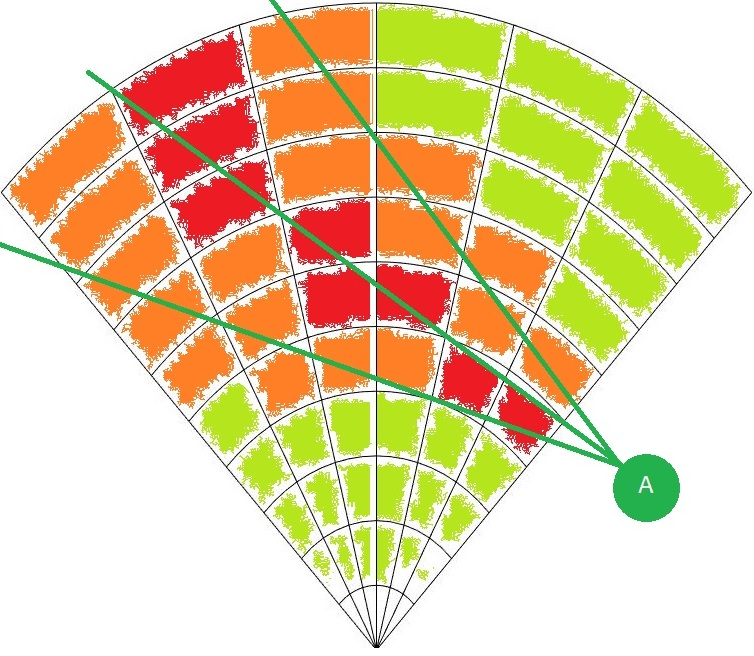
\includegraphics[width=0.7\textwidth]{\FIGDIR/TE052AdversaryProbabilitySpread}
    \caption{Intruder UAS intersection rate along the expected trajectory.}
    \label{fig:intruderProbabiltySpreadTheoretical}
\end{figure}   

\paragraph{Example of Intruder Intersection:} Let us neglect the \emph{time-impact} aspect on the \emph{intersection}.  The \emph{intruder} (black "I" circle) is intersecting one \emph{avoidance grid horizontal slice} (fig. \ref{fig:intruderProbabiltySpreadTheoretical}).  The intruder is moving along linear path approximation based on velocity (middle green line). The \emph{Horizontal Maneuver Uncertainty spread} is in \emph{green line boundary area} \emph{intruder intersection rating} is denoted as green-orange-red cell fill reflecting intersection severity:  red is a high rate of the intersection, orange is the medium rate of the intersection and green is a low rate of the intersection.
    


\paragraph{Moving Threats:} The \emph{UAS} can encounter following threats during the \emph{mission execution}:
\begin{enumerate}
    \item \emph{Non-cooperative Intruders} - the intruders who does not implement any approach to ensure mutual avoidance efficiency.
    
    \item \emph{Cooperative Intruders} - the intruders whom actively communicate or follow common agreed behavior pattern (ex. Rules of the Air).
    
    \item \emph{Moving Constraints} - the constrained portion of \emph{free} space which is shifting its boundary over time (ex. Short term bad weather).
\end{enumerate}
    
\begin{note}
    Our approach considers only \emph{UAS} intruders because \emph{Data Fusion} considers data received through \emph{ADS-B} messages. The \emph{Intruders} extracted from \emph{LiDAR} scan were not considered (ex. birds). The proposed \emph{intruder intersection models} are reusable for other \emph{intruder sources}.
\end{note}

\paragraph{Approach Overview:} The \emph{Avoidance Grid} (def. \ref{def:AvoidanceGrid}) is adapted to the \emph{LiDAR} sensor. The \emph{Euclidean grid intersections} are fairly simple. The \emph{polar coordinates grid} is not. The need to keep \emph{polar coordinates grid} is prevalent, because of fast \emph{LiDAR} reading assessment.  There are following commonly known methods to address this issue:

\begin{enumerate}
    \item\emph{Point-cloud Intersections} - the \emph{threat impact area} is discredited into a sufficiently thick point cloud. This point-cloud have \emph{point impact rate} and \emph{intersection time} assigned to each point. The \emph{point-cloud} is projected to \emph{Avoidance Grid}. If the \emph{impact point} hits $cell_{i,j,k}$ the cell`s impact rate is increased by the amount of \emph{point impact rate}. The final \emph{threat impact rate} in $cell_{i,j,k}$ is given when \emph{all} points from point cloud are consumed. Close point problem \cite{shamos1975closest} was solved by the application of method  \cite{bentley1980optimal}.
    
    \item\emph{Polygon Intersections} - the \emph{threat impact area} is modeled as a polygon, each $cell_{i,j,k}$ in \emph{Avoidance Grid} is considered as a \emph{polygon}. There is a possibility to calculate cell space geometrical inclusive intersection. The \emph{impact rate} is then given as rate between \emph{intersection volume} and $cell_{i,j,k}$ volume. The algorithm used for intersection selected based on:\citep{bentley1979algorithms} the selected algorithm  \emph{Shamos-Hoey} \cite{shamos1976geometric}.
\end{enumerate}

\begin{note}
    The \emph{Intruder Intersection} models are based on \emph{analytical geometry} for \emph{cones and ellipsoids} taken from \cite{sommerville2016analytical}.
\end{note}

    	\subsection{(R) Intruder Behaviour Prediction}\label{s:intruderBehaviourPrediction}
\paragraph{Idea:} \emph{Intruder Intersection Models} is about space-time intersection of \emph{intruder body} with \emph{avoidance Grid} and \emph{Reach Set}:
\begin{enumerate}
    \item The \emph{UAS} reach set defines \emph{time boundaries} to \emph{enter/leave} cell in avoidance grid.
    \item The \emph{Intruder} behavioral pattern defines \emph{rate} of \emph{space intersection} with cell bounded space in avoidance grid.
\end{enumerate}

The multiplication of \emph{space intersection rate} and \emph{time intersection rate} will give us \emph{intruder intersection} rate for our \emph{UAS} and intruder.


\paragraph{Intruder Dynamic Model:} The  definition of avoidance grid enforces the  most of these methods to be numeric. Let us introduce intruder dynamic model:

\begin{equation}\label{eq:intruderBasicLinearModel}
    \begin{aligned}
        \partial position /\partial time = velocity 
    \end{aligned}
    \quad | \quad
    \begin{aligned}
        position_x(t) = position_x(0) + velocity_x \times t\\
        position_y(t) = position_y(0) + velocity_y \times t\\
        position_z(t) = position_z(0) + velocity_z \times t
    \end{aligned}
\end{equation}

\noindent Position vector in euclidean coordinates $[x,y,z]$   is transformed into \emph{Avoidance Grid} coordinate frame. Velocity vector for $[x,y,z]$  is \emph{estimated and not changing}. The time  is in interval $[entry,leave]$, where $entry$ is intruder entry time into avoidance grid and $leave$ is intruder leave time from avoidance grid. 

\begin{note}
    If \emph{intruder} is considered, time of entry is marked as $intruder_{entry,k}$ where k is intruder identification, time of leave is marked as $intruder_{leave,k}$ where k is intruder identification. 
\end{note}

\paragraph{Cell Entry and Leave Times} $UAS_{entry}(cell_{i,j,k})$ and $UAS_{leave}(cell_{i,j,k})$ are depending on intersecting  \emph{Trajectories} and \emph{bounded cell space} (eq. \ref{eq:boundedSpaceCell}). There is \emph{Trajectory Intersection} function from (def. \ref{def:ContainedReducedReachSet}) which evaluates \emph{Trajectory segment} entry and leave time. 

The UAS \emph{Cell Entry} time is given as minimum of all \emph{passing trajectory segments} entry times (eq. \ref{eq:cellEntryTime}), if there is no \emph{passing trajectories} the UAS \emph{entry time} is set to 0.

\begin{equation}\label{eq:cellEntryTime}
    UAS_{entry}(cell_{i,j,k}) =  \min 
    \left\{\begin{aligned}
    0,en&try(Trajectory,cell_{i,j,k}):\\ &Trajectory\in Passing Trajectories
    \end{aligned}\right\}
\end{equation}

The UAS \emph{Cell Leave} time is given as maximum of all \emph{passing trajectory segments} entry times (eq. \ref{eq:cellLeaveTime}), if there is no \emph{passing trajectories} the UAS \emph{leave time} is set to 0.

\begin{equation}\label{eq:cellLeaveTime}
    UAS_{leave}(cell_{i,j,k}) =  \max 
    \left\{\begin{aligned}
    0,lea&ve(Trajectory,cell_{i,j,k}):\\ &Trajectory\in Passing Trajectories
    \end{aligned}\right\}
\end{equation}

\paragraph{Time Intersection Rate:} The key idea is to calculate how long the \emph{UAS} and \emph{Intruder} spends together in same space portion ($cell_{i,j,k}$). 
The \emph{Intruder} can spent some time in $cell_{i,j,k}$ bounded by interval of \emph{intruder} entry/leave time. 

The \emph{UAS} can spent some time, depending on \emph{selected trajectory} from \emph{Reach Set}. The time spent by UAS is bounded by entry (eq. \ref{eq:cellEntryTime}) and leave (eq. \ref{eq:cellLeaveTime}). 

The intersection duration of these two intervals creates \emph{time intersection rate} numerator, the \emph{maximal duration} of \emph{UAS} stay gives us \emph{denominator}. The \emph{time intersection rate} is formally defined in (eq. \ref{eq:timeIntersectionRate}). 

\begin{equation}\label{eq:timeIntersectionRate}
    time\left(\begin{gathered}UAS,\\Intruder,\\cell_{i,j,k}=\circ\end{gathered}\right)=  
    \frac{
        \left|
        \begin{gathered}
            \ [intruder_{entry}(\circ),intruder_{leave}(\circ)] \\
            \cap\\
            [UAS_{entry}(\circ),UAS_{leave}(\circ)]
        \end{gathered}\right|
        }
        {
        \left|\left[UAS_{entry}(\circ),UAS_{leave}(cell_{\circ})\right]\right|
        }
\end{equation}


\paragraph{Intruder Intersection Rate:} The \emph{Intruder Intersection Rate} (eq. \ref{eq:intruderIntersectionProbability}) is calculated as \emph{multiplication} of \emph{space intersection rate} (defined later) and \emph{time intersection rate} (eq. \ref{eq:timeIntersectionRate}).

\begin{equation}\label{eq:intruderIntersectionProbability}
    intruder\left(\begin{gathered}UAS,\\Intruder,\\cell_{i,j,k}\end{gathered}\right) = time \left(\begin{gathered}UAS,\\Intruder,\\cell_{i,j,k}\end{gathered}\right) \times space\left(\begin{gathered}UAS,\\Intruder,\\cell_{i,j,k}\end{gathered}\right)
\end{equation}

\begin{note}
    If there is no information to derive \emph{Intruder} entry/leave time for cells the \emph{time intersection rate} is considered 1.
\end{note}

The \emph{Intruder cell reach} time (eq. \ref{eq:intruderIntersectionTimeonPoint}) is bounded to discrete point in intersection model \cite{shamos1975closest,bentley1980optimal}. The intruder \emph{entry/leave time} is calculated similar to \emph{UAS cell entry (eq. \ref{eq:cellEntryTime})/leave (eq. \ref{eq:cellLeaveTime}) time}.

\begin{equation}\label{eq:intruderIntersectionTimeonPoint}
    point Reach Time(Intruder,point) = \frac{distance(Intruder.initial Position, point)}{|Intruder.velocity}
\end{equation}


\paragraph{Space Intersection Rate:} The \emph{Space Intersection Rate} reflects probability of \emph{Intruder} intersection with portion of space bounded by $cell_{i,j,k}$, to be precise with intruder trajectory or vehicle body shifted along the trajectory. The principles for \emph{space intersection rate} calculation are following:




\begin{enumerate}
    \item \textit{Line trajectory} - \emph{intruder} trajectory is given by linear approximation (eq. \ref{eq:intruderBasicLinearModel}), depending on \emph{intruder size} the intersection with avoidance grid can be:
    
    \begin{enumerate}[a.]
        \item \emph{Simple line} - intersection is going along the trajectory line line defined by intruder model (eq.\ref{eq:intruderBasicLinearModel}).
    
        \item \emph{Volume line} - intersection is going along the trajectory line defined by intruder model (eq. \ref{eq:intruderBasicLinearModel}) and intruder`s \emph{body radius} is considered in intersection.
    \end{enumerate}
    
    \item \emph{Elliptic cone} - initial position is considered as the top of a cone, the main cone axis is defined by intruder linear trajectory (eq. \ref{eq:intruderBasicLinearModel}) $time \in [0,\infty]$. The cone width is set by horizontal and vertical spread.
\end{enumerate}

    	\subsection{(W) Moving Constraints}\label{s:MovingVirtualConstraints}
\paragraph{Idea:} The basic ideas is the same as in case \emph{static constraints} (sec. \ref{s:virtualConstraints}). There is horizontal constraint and altitude constraint outlining the constrained space. The only additional concept is moving of \emph{constraint} on horizontal plane in global coordinate system. 

The constraint intersection  with \emph{avoidance grid} is done in \emph{fixed decision Time}, for cell in \emph{fixed cell leave time} (eq. \ref{eq:cellLeaveTime}), which means concept from static obstacles can be fully reused.

\paragraph{Definition:} The \emph{moving constraint definition} (eq. \ref{eq:movingConstraintDefinition}) covers minimal data scope for  moving constraint, assuming linear constraint movement. 

The original definition (eq. \ref{eq:staticConstraint}) is enhanced with additional parameters to support constraint moving:

\begin{enumerate}
    \item \emph{Velocity} - velocity vector on 2D horizontal plane.
    
    \item \emph{Detection time} - the time when \emph{constraint} was created/detected, this is the time when \emph center and boundary points position were valid.
\end{enumerate}

\begin{multline}\label{eq:movingConstraintDefinition}
    constraint = \{position,boundary,\dots\\\dots, velocity, detection Time, \dots \\\dots altitude_{start},altitude_{end}, safety Margin\}
\end{multline}

\paragraph{Cell Intersection:} The \emph{intersection algorithm} follows (eq. \ref{eq:contraintToCellIntersection}), only shift of the \emph{center and boundary points} is required. 

First let us introduce $\Delta time$ (eq. \ref{eq:deltatimeMovingconst}), which represents difference between the constraint detection time and expected cell leave time (eq. \ref{eq:cellLeaveTime}).

\begin{equation}\label{eq:deltatimeMovingconst}
    \Delta time = UAS_{leave}(cell_{i,j,k}) - detection Time
\end{equation}

\noindent The constraint boundary is shifted to:

\begin{multline}
    shifted Boundary(constraint) = \{new Point = point + velocity \times \Delta time:\dots\\\dots \forall point \in constraint.boundary \}
\end{multline}

\noindent The constraint center is shifted to:

\begin{equation}
    shifted Center(constraint) = constraint.center + velocity
\end{equation}

\begin{note}
    The $\Delta time$ is calculated separately for each $cell_{i,j,k}$, because \emph{UAS} is also  moving and reaching cells in different times. The \emph{cell leave time} can be calculated in advance after reach set approximation.
\end{note}

\paragraph{Alternative Intersection Implementation:} The alternative used for intersection selected based on polygon intersection algorithms review \citep{bentley1979algorithms}, the selected algorithm  is \emph{Shamos-Hoey} \cite{shamos1976geometric}.

The implementation was tested on \emph{Storm scenario} (sec. \ref{s:testStorm}) and it yelds same results.

   
    
    %Observations moved to Conclusion - no longer in use
    %\section{(W) Simulation Observations Summary}\label{sec:SimulationObservationsSummary}
    \noindent Use summary of this section in Conclusion and future work on specific 

\subsection{(W) Static Obstacles Avoidance}\label{sec:staticObstacleAvoidanceSummary}
    \noindent TODO: main points of building, slalom, maze scenarios - link artifacts and performance criteria

\subsection{(W) Constraints Avoidance}\label{sec:constraintAvoidanceSummary}
    \noindent TODO constraints main point, main loop processing, breach chance ? etc...
    
\subsection{(W) Unsupervised Intruder Avoidance}\label{sec:unsupervisedIntruderAvoidance}
    \noindent TODO emergency intruder avoidance emphasis navigation, Emergency avoidance contribution main points

\subsection{(W) Supervised (UTM) Intruder Avoidance}\label{sec:supervisedIntruderAvoidance}
    \noindent TODO UTM contribution main points
    
 

%% This adds a line for the Bibliography in the Table of Contents.
\addcontentsline{toc}{chapter}{Bibliography}
%% *** Set the bibliography style. ***
%% (change according to your preference/requirements)
%\bibliographystyle{plain}
%% *** Set the bibliography file. ***
%% ("thesis.bib" by default; change as needed)
\bibliography{thesis}

%% *** NOTE ***
%% If you don't use bibliography files, comment out the previous line
%% and use \begin{thebibliography}...\end{thebibliography}.  (In that
%% case, you should probably put the bibliography in a separate file and
%% `\include' or `\input' it here).

\end{document}
